\documentclass[11pt]{article}

\usepackage{graphicx}
\usepackage{wrapfig}
\usepackage{url}
\usepackage{wrapfig}
\usepackage{color}
\usepackage{marvosym}
\usepackage{enumerate}
\usepackage{subfigure}
\usepackage{tikz}
\usepackage{amsmath}
\usepackage{amssymb}
\usepackage{hyperref} 
\usetikzlibrary{automata, positioning}
\oddsidemargin 0mm
\evensidemargin 5mm
\topmargin -20mm
\textheight 240mm
\textwidth 160mm
\newcommand{\vw}{{\bf w}}
\newcommand{\vx}{{\bf x}}
\newcommand{\vy}{{\bf y}}
\newcommand{\vxi}{{\bf x}_i}
\newcommand{\yi}{y_i}
\newcommand{\vxj}{{\bf x}_j}
\newcommand{\vxn}{{\bf x}_n}
\newcommand{\yj}{y_j}
\newcommand{\ai}{\alpha_i}
\newcommand{\aj}{\alpha_j}
\newcommand{\X}{{\bf X}}
\newcommand{\Y}{{\bf Y}}
\newcommand{\vz}{{\bf z}}
\newcommand{\msigma}{{\bf \Sigma}}
\newcommand{\vmu}{{\bf \mu}}
\newcommand{\vmuk}{{\bf \mu}_k}
\newcommand{\msigmak}{{\bf \Sigma}_k}
\newcommand{\vmuj}{{\bf \mu}_j}
\newcommand{\msigmaj}{{\bf \Sigma}_j}
\newcommand{\pij}{\pi_j}
\newcommand{\pik}{\pi_k}
\newcommand{\D}{\mathcal{D}}
\newcommand{\el}{\mathcal{L}}
\newcommand{\N}{\mathcal{N}}
\newcommand{\vxij}{{\bf x}_{ij}}
\newcommand{\vt}{{\bf t}}
\newcommand{\yh}{\hat{y}}
\newcommand{\code}[1]{{\footnotesize \tt #1}}
\newcommand{\alphai}{\alpha_i}

\pagestyle{myheadings} 
\markboth{Homework 2}{Spring 2018 CS 475 Machine Learning: Homework 2}


\title{CS 475 Machine Learning: Project 2\\Supervised Classifiers 2\\
\Large{Due: Friday March 9, 2018, 11:59 pm}\footnote{Late submission deadline: Sunday March 11, 2018, 11:59 pm}\\
100 Points Total \hspace{1cm} Version 1.0}
\author{Junhao Xiong}
\date{}

\begin{document}
\large
\maketitle
\thispagestyle{headings}

\vspace{-.5in}


\section{Analytical (50 points)}

\paragraph{1) Decision Tree and Logistic Regression (10 points)}
Consider a binary classification task (label $y$) with four features ($x$):

\begin{tabular}{ |l|l|l|l|l| }
\hline
$x_1$ & $x_2$ & $x_3$ & $x_4$ & $y$ \\
\hline
 0& 1 & 1& -1 & 1 \\
 0&  1 & 1& 1 & 0 \\
 0&  -1 & 1& 1 & 1 \\
 0&  -1 & 1& -1 & 0 \\
\hline
\end{tabular}

\begin{enumerate}[(a)]
\item Can this function be learned using a decision tree? If so, provide such a tree (describe each node in the tree). If not, prove it.\\

Yes. This function is essentially y = $x_2$ XOR $x_4$, since $x_1$ and $x_3$ are uninformative features.\\

\begin{center}
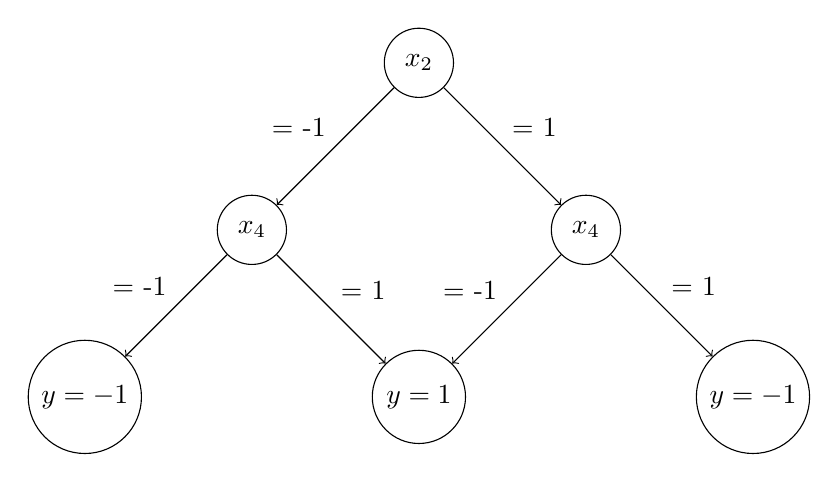
\begin{tikzpicture} [node distance = 3cm, on grid, auto]
\node[state] (x_2) {$x_2$};
\node[state] (x_2_isneg) [below left = of x_2] {$x_4$};
\node[state] (x_2_ispos) [below right = of x_2] {$x_4$};
\node[state] (y_neg_left) [below left = of x_2_isneg] {$y = -1$};
\node[state] (y_neg_right) [below right = of x_2_ispos] {$y = -1$};
\node[state] (y_pos) [below right = of x_2_isneg] {$ y = 1$};


\path[->] (x_2) edge node [swap] {= -1} (x_2_isneg);
\path[->] (x_2) edge node {= 1} (x_2_ispos);
\path[->] (x_2_isneg) edge node [swap] {= -1} (y_neg_left);
\path[->] (x_2_isneg) edge node {= 1} (y_pos);
\path[->] (x_2_ispos) edge node [swap] {= -1} (y_pos);
\path[->] (x_2_ispos) edge node {= 1} (y_neg_right);


\end{tikzpicture}
\end{center}

\item Can this function be learned using a logistic regression classifier? If yes, give some example parameter weights. If not, why not.\\

No. Logistic regression only works on linearly separable data. However, the given features are not linearly separable. To see the intuition of this, we can (pretend to) graph y on the plane $x_2$ vs $x_4$. y = 1 (let them be circles ) will land in the 2nd and 4th quadrants, y = -1 (let them be squares) will land in the 1st and 3rd quadrants. One can see, when attempt, that it is impossible to draw a line to separate the circles and squares. 

\item For the models above where you can learn this function, the learned model may over-fit the data. Propose a solution for each model on how to avoid over-fitting.\\

One can prune the decision tree. In particular, one can use the following new base cases for building the tree: stop when there are too few examples in a given branch; stop when a specified max depth is reached; stop when the classification error at a given level is not much worse than the error of its children. 

\end{enumerate}

\paragraph{2) Stochastic Gradient Descent (10 points)}
In the programming part of this assignment you implemented Gradient Descent. A stochastic variation of that method (Stochastic Gradient Descent) takes an estimate of the gradient based on a single sampled example, and takes a step based on that gradient. This process is repeated many times until convergence. To summarize:
\begin{enumerate}
\item Gradient descent: compute the gradient over all the training examples, take a gradient step, repeat until convergence.\\
\item Stochastic gradient descent: sample a single training example, compute the gradient over that training example, take a gradient step, repeat until convergence.
\end{enumerate}

In the limit, will both of these algorithms converge to the same optimum or different optimum? Answer this question for both convex and non-convex functions. Prove your answers.\\

Convex: both GD and SGD will converge to the same optimum, because GD and SGD both converge to local minima. In the case of convex functions, the local minima is the global minima. Hence, GD and SGD converge to the sam minima.\newline

Non-convex: GD and SGD will converge to the different optimums. Under reasonable assumptions of hyper-parameters, GD follows the direction of steepest descent and converges to the local minima of the neighborhood. On the other hand, since SGD calculates the gradient based on a single example, its direction of descent is not necessarily the steepest. it may leave the starting neighborhood and converge to the local minima of a different neighborhood.


\paragraph{3) Kernel Trick (10 points)}
The kernel trick extends SVMs to learn nonlinear functions. However, an improper use of a kernel function can cause serious over-fitting. Consider the following kernels.
\begin{enumerate}[(a)]
\item Inverse Polynomial kernel: given $\|x\|_2\leq 1$ and $\|x'\|_2\leq 1$, we define $K(x, x') = 1/(d-x^\top x')$, where $d\geq 2$. Does increasing $d$ make over-fitting more or less likely?\\

Increasing $d$ makes over-fitting less likely. Since $-1 \leq x^\top x' \leq 1$, so we have $1/(d+1) \leq K(x, x') \leq 1/(d-1)$. Now consider a small $d$, e.g. $d = 2$, then $1/3 \leq K(x, x') \leq 1$; a large d, e.g. $d = 100$, then $1/101 \leq K(x, x') \leq 1/99$. Note that the range for $K(x, x')$ is larger in the case of smaller d, which means the kernel value, thus the weights learn, are more likely to fit to the extremes of the data, making overfitting more likely.


\item Chi squared kernel: Let $x_j$ denote the $j$-th entry of $x$. Given $x_j>0$ and $x_j'>0$ for all $j$, we define $K(x, x') = \exp\left(-\sigma\sum_j\frac{(x_j-x'_j)^2}{x_j+x'_j}\right)$, where $\sigma>0$. Does increasing $\sigma$ make over-fitting more or less likely?\\

Increasing $\sigma$ makes overfitting more likely. When $\sigma$ is very large, e.g. 1000, if $x_j$ and $x_j'$ are slightly different from each other, $K(x, x')$ will tend to zero. Thus, the weights learned by SVM will overfit to a small neighborhood of points. When $\sigma$ is very small, e.g. 1, then $K(x, x')$ is likely to be nonzero for a larger neighborhood of points, thus reducing over-fitting. 

\end{enumerate}
We say $K$ is a kernel function, if there exists some transformation $\phi:\mathbb{R}^m\rightarrow \mathbb{R}^{m'}$ such that $K(x_i,x_{i'}) = \left<\phi(x_i),\phi(x_{i'})\right>$.
\begin{enumerate}[(c)]
\item Let $K_1$ and $K_2$ be two kernel functions. Prove that $K(x_i,x_{i'}) = K_1(x_i,x_{i'}) + K_2(x_i,x_{i'})$ is also a kernel function.\\

Recall that $K$ is a kernel (function) if $K$ (matrix) is symmetric and positive semidefinite.
	\begin{equation*}
		z^\top K z = z^\top (K_1 + K_2) z = z^\top K_1 z + z^\top K_2 z  \text{	by distributivity of matrix multiplication}
	\end{equation*}
	
Since $K_1$ and $K_2$ are kernels, they are positive semidefinite, so both terms in the sum above are nonnegative, so $z^\top K z$ must be nonnegative. Hence $K$ is positive semidefinite.\\
Moreover, since $K_1$ and $K_2$ are symmetric, $K$ is clearly symmetric. Hence $K$ is a kernel matrix, as well as a kernel function. 

\end{enumerate}

\paragraph{4) Dual Perceptron (8 points)} 
\begin{enumerate}[(a)]
\item You train a Perceptron classifier in the primal form on an infinite stream of data. This stream of data is not-linearly separable. Will the Perceptron have a bounded number of prediction errors?
Since Perceptron can only separate linearly separable data, with an infinite stream of data, Perceptron will have unbounded number of prediction error. 

\item Switch the primal Perceptron in the previous step to a dual Perceptron with a linear kernel. After observing $T$ examples in the stream, will the two Perceptrons have learned the same prediction function?
	\begin{equation*}
		\text {The primal prediction function is: } \hat{y} = sign(w^\top x) = sign(\sum_i y_i x_i I_{\text{ith example is misclassified}} \cdot x )
	\end{equation*}
where I is an indicator function.  But this can also be written as:
	\begin{equation*}
		sign(\sum_i \alpha_i y_i x_i \cdot x)
	\end{equation*}
which is the dual formulation of Perceptron. Given a linear kernel $K$, i.e. $K(x, x') = x \cdot x'$. Hence the above equation can also be written as:
	\begin{equation*}
		sign(\sum_i \alpha_i y_i K(x_i, x))
	\end{equation*}
This is the dual formulation of Perceptron with linear kernel. Hence we have shown that the primal and dual Perceptron learn the same prediction function.  

\item What computational issue will you encounter if you continue to run the dual Perceptron and allow $T$ to approach $\infty$? Will this problem happen with the primal Percepton? Why or why not?\\

For the dual Perceptron, we need to keep track of an $\alpha$ for each training example we misclassify. Since the dual Perceptron also has unbounded prediction error, we will have an unbounded number of $\alpha$ as $T$ approaches $\infty$. But with primal form, we only keeps track of the weights, whose length is bounded by the length of $x$, so it would not encounter the same problem. 

\end{enumerate}


\paragraph{5) Convex Optimization (12 points)}
Jenny at Acme Inc. is working hard on her new machine learning algorithm. She starts by writing an objective function
that captures her thoughts about the problem. However, after writing the program that optimizes the objective
and getting poor results, she returns to the objective function in frustration. Turning to her colleague Matilda,
who took CS 475 at Johns Hopkins, she asks for advice. ``Have you checked that your function is convex?'' asks Matilda.
``How?'' asks Jenny.
\begin{enumerate}[(a)]
\item Jenny's function can be written as $f(g(x))$, where $f(x)$ and $g(x)$ are convex, and $f(x)$ is non-decreasing. Prove that $f(g(x))$ is a convex function. (Hint: You may find it helpful to use the definition of convexity. Do not use gradient or Hessian, since $f$ and $g$ may not have them.)\\

Since g is convex we have:
	\begin{equation*}
		g(tx + (1-t)y) \leq t g(x) + (1-t) g(y) 
	\end{equation*}

Since f is nondecreasing:
	\begin{equation*}
		f(g(tx + (1-t)y)) \leq f(t g(x) + (1-t) g(y)) 
	\end{equation*}

Since f is convex:
	\begin{equation*}
		f(t g(x) + (1-t) g(y)) \leq t f(g(x)) + (1-t) f(g(y))
	\end{equation*}
	
Hence we have:
	\begin{equation*}
		f(g(tx + (1-t)y)) \leq t f(g(x)) + (1-t) f(g(y))
	\end{equation*}
	
This shows $f(g(x))$ is a convex function.
	
\item Jenny realizes that she made an error and that her function is instead
$f(x)-g(x)$, where $f(x)$ and $g(x)$ are convex functions. Her objective may or may not be convex. Give examples of functions $f(x)$ and $g(x)$ whose difference is convex, and functions $\bar{f}(x)$ and $\bar{g}(x)$ whose difference is non-convex.
\end{enumerate}

Let $f(x) = x^2$ , $g(x) = 2 x^2$. Then $f(x) - g(x) = -x^2$, which is concave, i.e. not convex.\\

Let $\bar{f}(x) = 2 x^2$ and $\bar{g}(x) = x^2$. Then $\bar{f}(x) - \bar{g}(x) = x^2$, which is convex.\\

\begin{enumerate}[(a)]
\setcounter{enumi}{2}
\item Why was Jenny getting poor results with a non-convex function?

Because for non-convex function, local optimum is not necessarily global minimum. When Jenny optimize for a non-convex loss function, she is not guaranteed to reach the global minimum of the loss function. When the objective function is not minimized properly, the results will be poor.

\item One approach for convex optimization is to iteratively compute a descent direction and take a step along that direction to have a new value of the parameters. The choice of a proper stepsize is not so trivial. In gradient descent algorithm, the stepsize is chosen such that it is proportional to the magnitude of the gradient at the current point. What might be the problem if we fix the stepsize to a constant regardless of the current gradient? Discuss when stepsize is too small or too large.
\end{enumerate}

If we fix the stepsize to be too small, we will converge very slowly, since the weights will be updated only slightly every time. If we fix the stepsize to be too large, we might overshoot when we are close to the optimum.  


\end{document}
